\documentclass[11pt]{article}
\usepackage{geometry}                
\geometry{letterpaper}                   

\usepackage{graphicx}
\usepackage{amssymb}
\usepackage{epstopdf}
\usepackage{natbib}
\usepackage{amssymb, amsmath}
\DeclareGraphicsRule{.tif}{png}{.png}{`convert #1 `dirname #1`/`basename #1 .tif`.png}

%\title{Title}
%\author{Name 1, Name 2}
%\date{date} 



%%%%%%%%%%%%%%%%%%%%%%%%%%%%%%%%%%%%%%%%%%%%%%%%%%%%%%%%%%%%%%%%%%%%%%%%%%%%%%%%%%%%%%%%%%%%%%%%%%%%%%%%%%%% 
%Additinal packages ants in the pants
%%%%%%%%%%%%%%%%%%%%%%%%%%%%%%%%%%%%%%%%%%%%%%%%%%%%%%%%%%%%%%%%%%%%%%%%%%%%%%%%%%%%%%%%%%%%%%%%%%%%%%%%%%%%
\usepackage{float}
\usepackage[]{algorithm2e}
\usepackage{todonotes}
\usepackage[german]{babel}
\usepackage[utf8]{inputenc}	
%-------------------------------------Listings------------------------------------- 				
\usepackage{listings}	
\lstset{
language=matlab,
basicstyle=\sffamily\scriptsize,
frame=single,
rulecolor=\color{gray},
numbers=right,
stepnumber=5,
firstnumber=1,
numberfirstline=true,
xrightmargin= 20pt, 		%Abstand vom Rahmenrechts
framexrightmargin=20pt,	%Abstand der Nummern
%xleftmarargin= 25pt, %Abstand links
numberstyle=\sffamily\scriptsize\color{lightgray}
%numberstyle=\sffamily\tiny\color{lightgray}
%columns=flexible,
%keepspaces=true,
} 


%\renewcommand{\figurename}{Bild}


%\addto\captionsngerman{\renewcommand{\figurename}{Bild}}













\begin{document}
\pagenumbering{roman}
\renewcommand{\figurename}{Figure}


\thispagestyle{empty}

\begin{center}
\includegraphics[width=5cm]{ETHlogo.eps}

\bigskip


\bigskip


\bigskip


\LARGE{ 	Lecture with Computer Exercises:\\ }
\LARGE{ Modelling and Simulating Social Systems with MATLAB\\}

\bigskip

\bigskip

\small{Project Report}\\

\bigskip

\bigskip

\bigskip

\bigskip


\begin{tabular}{|c|}
\hline
\\
\textbf{\LARGE{Dessert ant Adaptive orientation of dessert ants }}\\
\textbf{\LARGE{(lateinischer Name)}}\\
\\
\hline
\end{tabular}
\bigskip

\bigskip

\bigskip

\LARGE{Florian Hasler, Matthias Heinzmann,
\\ Andreas Urech,  Dominik Werner}



\bigskip

\bigskip

\bigskip

\bigskip

\bigskip

\bigskip

\bigskip

\bigskip

Zurich\\
December 2015\\

\end{center}



\newpage

%%%%%%%%%%%%%%%%%%%%%%%%%%%%%%%%%%%%%%%%%%%%%%%%%

\newpage
\setcounter{page}{1}
\section*{Agreement for free-download}
\bigskip


\bigskip


\large We hereby agree to make our source code for this project freely available for download from the web pages of the SOMS chair. Furthermore, we assure that all source code is written by ourselves and is not violating any copyright restrictions.

\begin{center}

\bigskip


\bigskip

\begin{tabular}{@{}p{3.3cm}@{}p{6cm}@{}@{}p{6cm}@{}}
\begin{minipage}{3cm}

\end{minipage}
&
\begin{minipage}{6cm}
\large Florian Hasler
\end{minipage}
&
\begin{minipage}{6cm}
\large Matthias Heinzmann
\end{minipage}
\end{tabular}
\ \\
\ \\
\ \\
\ \\
\ \\
\ \\
\ \\
\begin{tabular}{@{}p{3.3cm}@{}p{6cm}@{}@{}p{6cm}@{}}
\begin{minipage}{3cm}
\end{minipage}
&
\begin{minipage}{6cm}
\large Andreas Urech
\end{minipage}
&
\begin{minipage}{6cm}
\large Dominik Werner
\end{minipage}
\end{tabular}
\end{center}
\newpage

%%%%%%%%%%%%%%%%%%%%%%%%%%%%%%%%%%%%%%%



% IMPORTANT
% you MUST include the ETH declaration of originality here; it is available for download on the course website or at http://www.ethz.ch/faculty/exams/plagiarism/index_EN; it can be printed as pdf and should be filled out in handwriting


%%%%%%%%%% Table of content %%%%%%%%%%%%%%%%%

\tableofcontents

\newpage

%%%%%%%%%%%%%%%%%%%%%%%%%%%%%%%%%%%%%%%

%\setcounter{page}{1}
\pagenumbering{arabic}
\section{Abstract}
The Saharan Desert ant (Cataglyphis Fortis) lives under harsh environmental conditions which make a sophisticated way of orientation necessary.\\
German biologist Wehner \cite{Wehner2003},\cite{Wehner1988}, \cite{Wehner1998} has proposed two such means. Namely path integration and orientation by landmarks.
In his final conclusion he considers both methods important and assumes that the ant has a way of adopting the priority of each mechanism according to the current situation.\\
\ \\
 In previous years a group called gordonteam\cite{GordonTeam2008} already implemented a model based on the before mentioned articles. In their report they noted that their path integration did not work and that they were not able to combine all methods. Our plan is to extend upon their work and fix the problem with the path integrator as well as to bind the two methods together. 

\newpage
\section{Individual contributions}
We split up the work among the members of our group based upon their past experience in various topics and skills needed to develop the project. 
In order for every member to understand the project in its entirety we held meetings once a week where every member presented his work to the rest of the group. In those meetings we also discussed how to proceed with the project.
We divided the work as follows:
\begin{itemize}
\item Path integrator: Florian Hasler, Matthias Heinzmann
\item Landmarks: Matthias Heinzmann
\item Multi foodsource support: Dominik Werner
\item Software Architecture: Florian Hasler, Matthias Heinzmann,Dominik Werner
\item Timer: Andreas Urech
\item Ant looking around behaviour: Florian Hasler
\item Project report: Andreas Urech, Florian Hasler, Matthias Heinzmann, Dominik Werner
\item \LaTeX - version of report and presentation: Andreas Urech
\end{itemize}

\section{Introduction and Motivations}
 Due to the sparse Saharan resources the ants have to use them economically. Due to this fact the weight of the ant's brain is only around 0.1mg. It is not possible for a brain this small to execute calculations of high complexity. They have to rely on simple but efficient ways to be able to keep track of their individual position. Our goal of implementing a model of the ants navigation system will hopefully show if the proposed model can reproduce the behavior observed in real ants.
Our main question is:\\
\textit{
Is the path integrator-model proposed by Wehner1988 \cite{Wehner1988} to describe the ant's behaviour in one specific scenario applicable for more general situations?\\
Further questions are:
\begin{itemize}
\item Are we able to predict what happens if we alter the environment? (depends on the question beforehand) 
\item Can the ants survive if we rid the environment completely of any landmarks? 
\end{itemize}
}

\section{Description of the Model}
\subsection{Orientation}
As mentioned the desert ant's main means of orientation are:
\begin{itemize}
\item pathintegration
\item local landmark orientation
\end{itemize}
The cataglyphis doesn't communicate with its conspecifics on a foraging walk.
This is because the prey usally consists of small parts of insects, that can be carried by one ant, and no need for sharing information arises. [Appendix \ref{Sec:Correspondence}]




\subsubsection{Pathintegration}\label{Sec:PathIntegration}
No matter the random way out of its nest, the ant is able to return in a more or less straight line. This remarkable ability is reached by pathintegration. Therefore the ant is always aware in which direction its nest is located. These calculations are executed with imperfections which accumulate with growing path length. In extreme cases pathintegration causes the ant to miss its nest and other means of orientation are necessary. \\
In Wehner1988\cite{Wehner1988}\footnote{on page 5288} the following formulas have been derived, which give a rough approximation of the ants pathintegration.
\begin{align*}
\varphi(n+1) =& \varphi(n) +k \cdot \frac{(\pi +\delta)\cdot(\pi-\delta)\cdot \delta}{l(n)}\\
l(n+1) =& l(n) +1 -\frac{|\delta|}{\pi}
\end{align*}
where $k=0.1316$ is a fitting constant Wehner1988 \cite{Wehner1988}, $\delta$ is the angle between the current walking direction (thick line in figure \ref{fig:Delta}) and an artificial line back to the nest.The step width is assumed to be 1.

\begin{figure}[H]
\centering
\includegraphics[scale=1]{./Pics/delta.png} 
\caption{Angle $\delta$ \label{fig:Delta} }
\end{figure} 





%In the following we will discuss the quality of this specific path integrator model.
%Let’s assume that the ant is currently at a position $l = L$ and $\varphi = 0$ (we can assume $\varphi = 0$ without loss of generality because if $\varphi ~= 0$ we would simply rotate our coordinate system to obtain $\varphi’ = 0$ again). Furthermore, the global vector at this point is assumed to be perfect, which means that it directly points from the nest to the ant’s position. 
%Now the ant does one step with a specific step width $l$. The direction is given by the turning angle delta which is assumed to be normal distributed with $\mu = 0$ and $\sigma = \frac{\pi}{16}$.  
%The plot of the expected error of the global vector in this one step can be seen in the figure below.
%\begin{figure}[h]
%\centering
%\includegraphics[scale=0.7]{./Pics/path integrator_error_plot.png} 
%\caption[Pathintegrator Error]{Pathintegrator Error}
%\end{figure} \\

%It can easily be observed that the distance from the nest L has almost no influence on the error expect for very small distances (0m – 2m). The performance of the global vector model is rather influenced by the choice of the step width $l$. According to the figure, the step width should be chosen sufficiently small.\\
\ \\
%By varying the step width we end up with a new problem. The path the ant walks along is strongly influenced by the choice of the step width. But what we would like to have is that the ant walks in a similar way no matter what the step size is. 
%To address this problem we set the variance in the distribution of the turning angle theta in relation to $dt$ (step width $l$ of the ant is determined by $l = dt\cdot antSpeed$). 
%We made the following ansatz:\\
%$\sigma(dt) = dt^{c}  \sigma_{0}$ with $c \in (0,1]$ and $\sigma_{0}$ the standard deviation for $dt = 1$.
%Then we let the ant do $n1=1$ steps with $dt=1$ and $n2=\frac{1}{dt}$ steps with some $dt \in (0,1]$. Finally we correlated the resulting positions of the two situations and looked for the best correlation, i.e. $c$ such that the difference between the two situations is lowest. 
%The result for a normal distribution with $\mu =0$ and $\sigma_{0} = \frac{\pi}{12}$ and $dt = 0.1$ can be seen in the figure below.

%\begin{figure}[H]
%\centering
%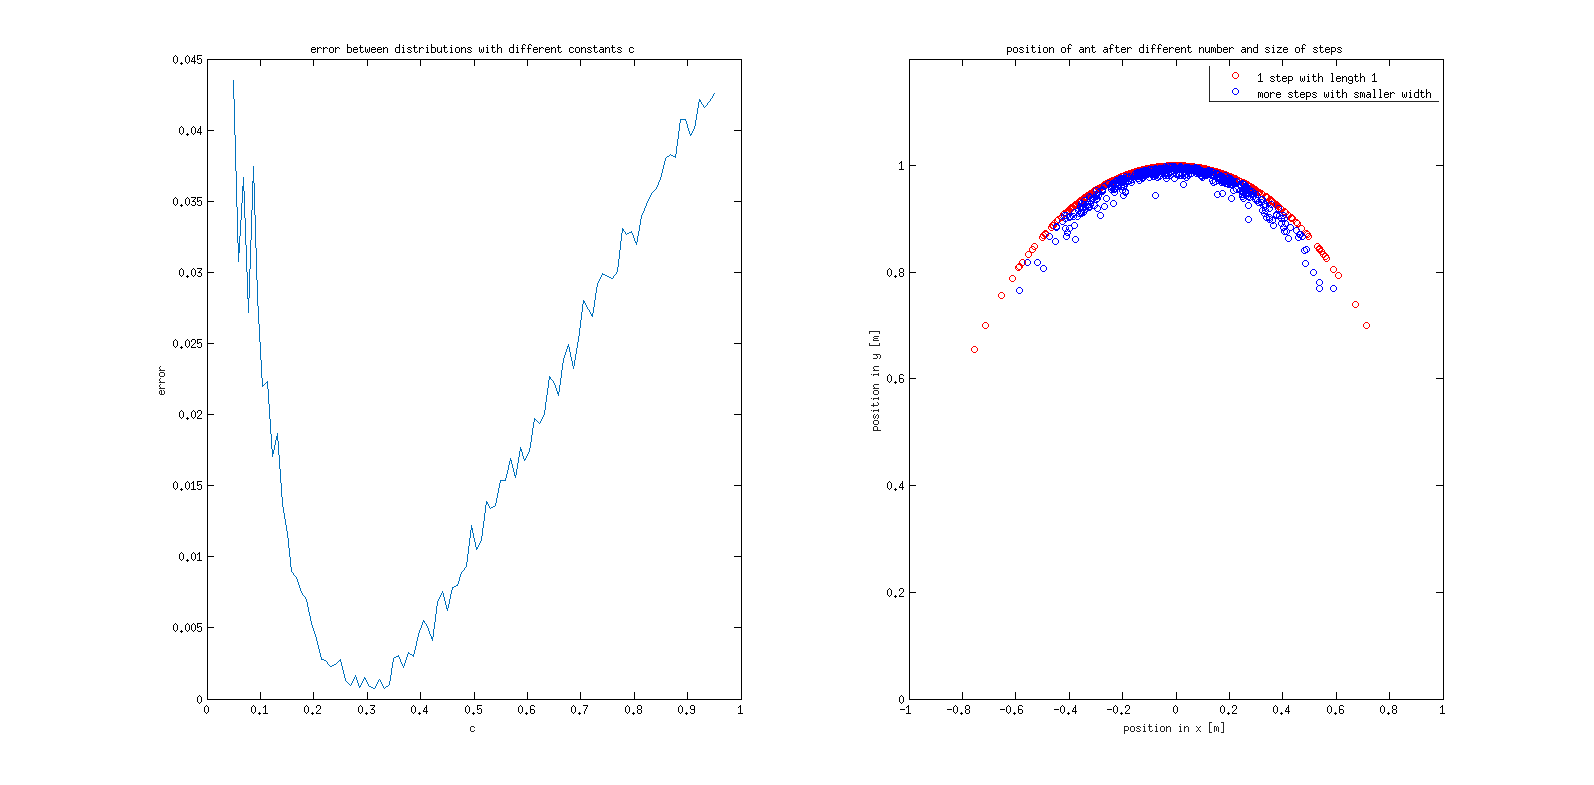
\includegraphics[scale=0.36]{./Pics/VarianceForStepWidth_plot.png} 
%\caption[VariacneForStepWidth]{VarianceForStepWidth}
%\end{figure} 
%Afterwards we tried out several different $dt’s$ and $\sigma_{0}’s$ but the result for $c$ was always similar to the one in the left side of the figure. The value for the best fitting $c$ can be read off as being approximately 0.3.


\subsubsection{Local landmark Orientation}
Desert ants can associate familiar landmarks with a local vector, which can lead them directly from one place to the visual catchment area of the next one (Wehner2003 \cite{Wehner2003}). Therefore, as soon as an ant recognizes a landmark it knows where to go to reach the next landmark or the nest respectively given that it has already familiarized with this landmark.  
For our implementation, we simplified this ability, i.e. the local vector, in the following way. 
As soon as the ant sees a landmark it goes there. When arrived, the ant walks $N$ steps in a direction $d$ where $N$ and $d$ are determined by the landmark’s properties. Like that, the local vector is implicitly defined by $N$ and $d$. The ant reaches the next landmark or the nest respectively after having walked along the local vector. 
For simplicity’s sake, we assumed that all landmarks are familiar to all ants at the start of our simulation.





\subsection{Combination} \label{Sec:Combination}
%It is not that the various means of orientations are combined in a weighted fashion. Given certain criteria the different means are used separately.\\
The results gained by R. Wehner's experiments indicate that ants use predominantly path integration, but if available using local landmarks is more preferable. It has been concluded that the ant transiently inhibits the global vector when being in familiar territory. The global vector reemerges after the local vector ceases. Whilst navigating via the local vector the global vector is continuously updated.
\\ \

\begin{algorithm}[H]

  \SetKwFunction{algo}{ReturnToMyNest}
  \SetKwProg{myalg}{Algorithm}{}{}
  \myalg{\algo{}}{




%\SetKwFunction{goToMyNest}{goToMyNest}
%\goToMyNest
 \While{not at nest}{ 
 execute global vector;\\
 update global vector;
 
  \If{local vector recognised}{
   		\While{local vector $ > 0$}{
   		 execute local vector\;
   		 update local vector\;
   		 update global vector;
   			}
		}
}
 \Return
 } 
\caption{Returning to the nest}
\end{algorithm}







\newpage

\section{Implementation}
For our simulation we will use an agent based model where every agent will be representing an ant. To be able to compare our model with the real world data we have to keep track of several different variables:
\begin{description}
\item[nestLocation:] This is a 2D vector which indicates the position of the nest inside a sand pan.
\item[foodSourceLocation(s): ]These 2D vectors symbolize the location of a food source which the ant will have to travel to. It should be possible to implement an ephemeral (non-renewable) food source so the ant has to look for a new one if the first does not yield food anymore.
\item [ants: ]The agents themselves who contain their position data and other information to track the simulation.
\item[landmarks:]Objects that symbolize visual orientation points for the ants.
\end{description}
\ \\
To implement our agent based model we decided to use object orientated programming because it
seemed more intuitive than a procedural approach in this case.
\subsection{UML-Diagram}
The following graphic shows the UML-Class diagram that describes the data model of our project.
The files run.m, updateGround.m, vector2angle.m and distanceBetweenTwoPoints.m are not part of
this diagram since they are procedural functions and not classes.
\begin{figure}[h]
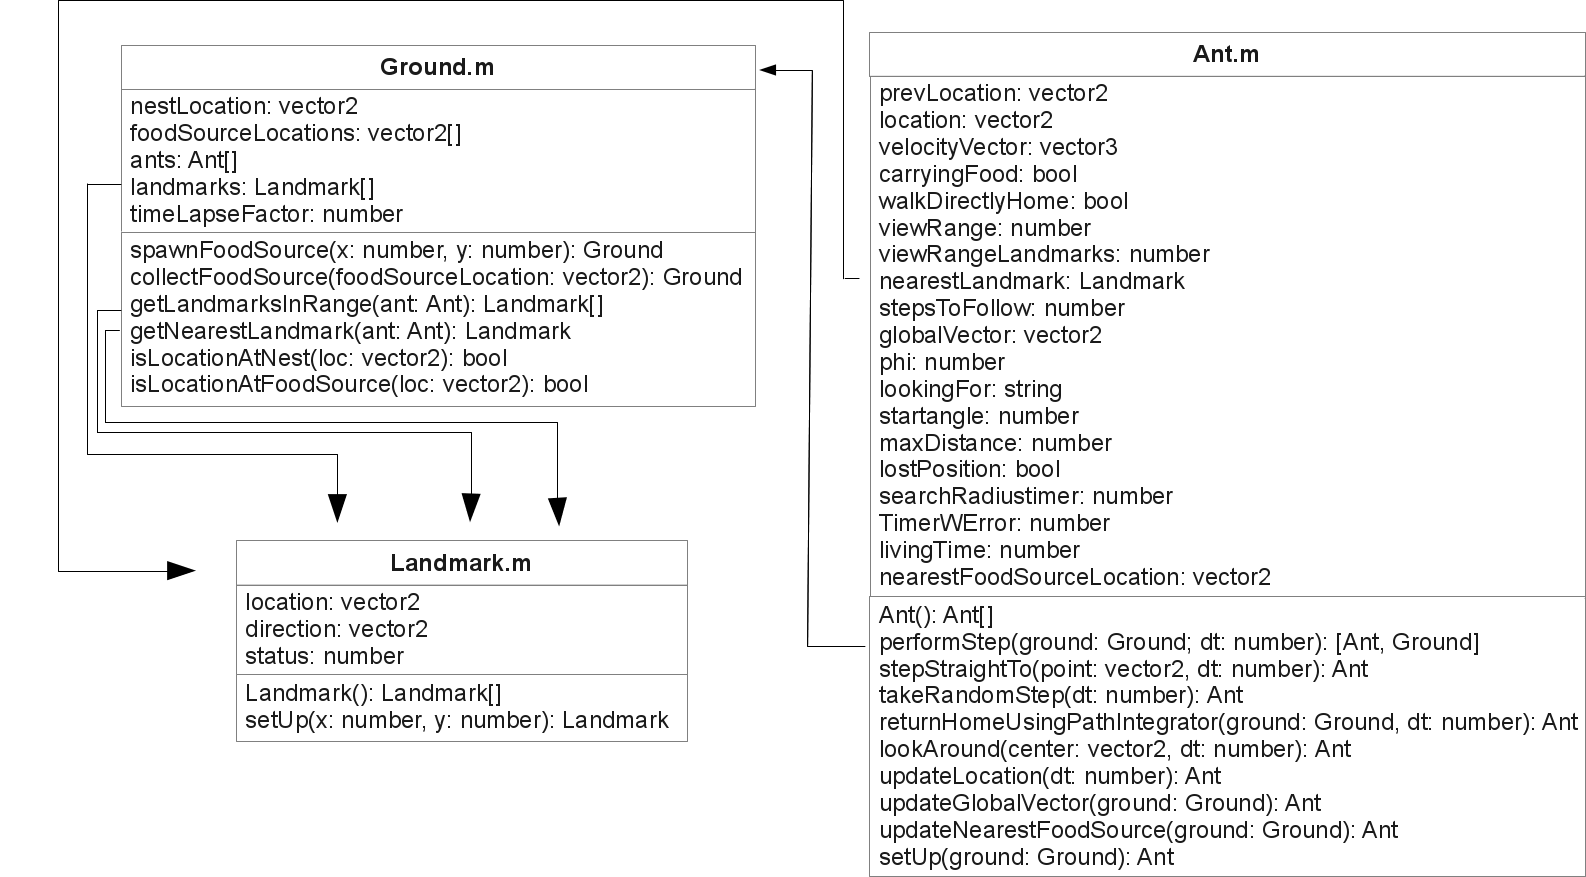
\includegraphics[scale=0.35]{./Pics/uml.png} 
\caption[UML]{UML}
\end{figure} \\
This diagram shows the classes of the project and how they are related. Since Matlab does not
support information hiding the public/private information is missing in the diagram. Because
 Matlab uses matrices in many cases all data-types with the exceptions of bool, string, Ant, Ground
and Landmark are matrices of type double \footnote{ Mathworks2015\cite{Mathworks2015}}  as entries:
\begin{itemize}
\item vector2: double(2,1)
\item vector3: double(3,1)
\item vector2[]: double(2, n)
\item number: double(1,1)
\end{itemize}
Something else to be mentioned is that Matlab does not make use of pointers but instead copies
instances of objects and does not alter the original. This means that in order for a method that is
supposed to alter an object the original object has to be overwritten. This can be done by letting
methods return the object that is containing them (this).

\lstinputlisting[captionpos=b,caption=copies,label="copies"]{./Code/copies.m}
For this reason nearly every method does return the object it belongs to as a result.

\subsection{Source Code}
To shed some light on how we implemented the model we will quickly describe the source code.
The object orientated approach made it possible to implement new ideas relatively fast at the correct
location.
\subsubsection{run.m}
[Listing \ref{"list:run.m"} in \ref{run}].This file does all the parametrization and executes the setup methods of the various classes utilized
in this project. It is supposed to be used as an easy way to alter the setup if the need arises.\\
The file contains the before mentioned setup section, followed by the execution section where the
main-loop does update the ground and the ants objects. Also inside of the main-loop one can find
the time handling. At the beginning of each iteration a timestamp is saved and then used at the end
of the iteration to pause the execution in order to have a uniform speed throughout the running time
of the program.\\
The last section of the file does handle callback-functions from the user interface. The user interface
in our case is the plot that opens and displays the various agents moving in the world. The user
interface provides the following functions:

\begin{itemize}
\item \textbf{Spawn new food source:} New sources of food for the ants to collect can be spawned by
simply clicking at the location in the world were the source should appear.
\item \textbf{Close:} In order for the program to terminate without errors we used a callback-function
from closing event of our plot-figure to terminate the program.
\end{itemize}








\subsubsection{distanceBetweenTwoPoints.m}
[Listing \ref{"distanceBetweenTwoPoints.m"} in \ref{distancebetweenTwoPoints}]. A simple helper function which calculates the distance between two points.


\subsubsection{vector2angle.m}
[Listing \ref{"list:vector2angle.m"} in \ref{vector2angle}]. This helper function calculates the angle of a given vector in radians. The value of the result ranges from 0 to 2 pi. This is important in order for the path integrator to work correctly. Additional corrections (to use the acute and not obtuse angle) are done in Ant.m. 


\subsubsection{updateGround.m}
[Listing \ref{"list:updateGround.m"} in \ref{updateGround}]. This function does not change anything on the Ground object as its name might suggest. This
method does update the plot and redraws all ants, food sources, the nest and the landmarks.


\subsubsection{Landmark.m}
[Listing \ref{"list:Landmark.m"} in \ref{Landmark}]. This class represents a visual landmark. It is defined as having a location, a direction vector a status which is represented by a bool and steps to follow which determines how many steps has to take after the landmark. The direction vector is used by incoming ants to leave the
landmark in the direction provided by the landmark. This is supposed to mimic the ants procedural
memory.

\subsubsection{Ground.m}
[Listing \ref{"list:Ground.m"} in \ref{Ground}]. This class serves as container for all agents and the objects they can interact with. Besides its function as a container it also provides methods to spawn new food sources and landmarks in the world as well as various methods which can determine the proximity of a certain target. 


\subsubsection{Ant.m}
[Listing \ref{"List:Ant.m"} in \ref{Ant}].This class represents our agent and implements the mathematical model proposed by R. Wehner \cite{Wehner1988}. The model is implemented pretty straight forward with a few exceptions. Because
our ants aren't real and do not have a limited field of view but can see 360 degrees we had to create
a property which tells the ant if it is leaving the nest so it doesn't immediately go back to the nest
after it left it. This is due to the assumption that foraging ants that come across their nest during
their searches, reset their global vector to correct errors or in other words, they will use the local
vector rather than the global vector (as described in  \ref{Sec:Combination}) . Furthermore we have a severe mathematical problem
when we are near the nest. Because we divide by the length of our global vector we cause a division
by zero in our update method once the global vectors length becomes zero. To avoid this we
actually wait until the nest is outside of the ants view distance and set the length of the global vector
to the view distance. It is reasonable to assume that the real ants do something similar because of
the before mentioned local vector.\\
\ \\
Also important is the method that takes a random step. For that, the ant randomly chooses the angle which it turns its direction in the next step out of a probability distribution with expected value $0$ and variable variance $\sigma_{0}^{2}$. \\
\ \\
As described above the ants vision was simplified for the implementation and a field of view is not
implemented. Once the ant is within view distance of an object (food source, landmark, nest) it
steps straight towards it (local vector). The decision if the ant has reached its target is made by
checking the length of the difference vector between the ant's location and the target. Once the
length is smaller than a certain threshold value the ant has reached its target. Since it is possible to
have many different food sources as well as landmarks we implemented methods which update the
properties nearestFoodSourceLocation and nearestLandmark. Those two properties are then used
for the comparison. It is also important to note that the landmarks are visible from further away than
food sources or the nest.\\
\ \\
Real ants cannot stay outside for too long because they would die in the heat of the desert. We
implemented a timer that every ant updates (with a small, random error) which tells the ant when it
has to return to the nest during its search for food. If an ant does not reach the nest in time it will
stop moving thus being dead.









%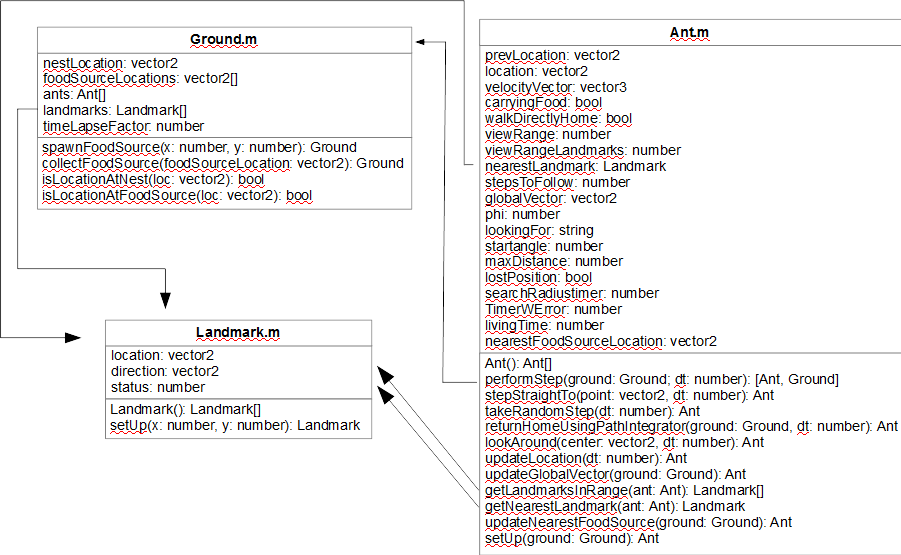
\includegraphics[width=5cm]{uml.png}



%\lstinputlisting[captionpos=b,caption=Beispiel,label="Label_Beispiel"]{./Code/Beispiel.m}

\section{Simulation Results and Discussion}
\subsection{Discussion of the Pathintegrator}
The general idea of the path integrator is described in section \ref{Sec:PathIntegration}. In the following we will discuss the quality of this specific path integrator model.
Let’s assume that the ant is currently at a position $l = L$ and $\varphi = 0$ (we can assume $\varphi = 0$ without loss of generality because if $\varphi \approx 0$ we would simply rotate our coordinate system to obtain $\varphi’ = 0$ again). Furthermore, the global vector at this point is assumed to be perfect, which means that it directly points from the nest to the ant’s position. \\
Now the ant does one step with a specific step width $l$. The direction is given by the turning angle $\delta$ which is assumed to be normal distributed with expectation value $\mu$ and standard deviation $\sigma = \frac{\pi}{16}$ where $\mu$ corresponds to the direction the ant has been walking in the previous step. Of course, the path integrator critically depends on this $\mu$ as can be seen in figure \ref{fig:PathintegratorError} (plots for $\mu=0,40,80,120^{\circ}$). In figure \ref{fig:PathintegratorError}, the first row illustrates the absolute expected error of the path integrator while the second row illustrates the expected error relative to the step width l.
\begin{figure}[H]
\centering
\includegraphics[scale=0.31]{./Pics/Pathintegrator_error_plot.png} 
\caption{Pathintegrator error \label{fig:PathintegratorError} }
\end{figure} 
One can easily observe in figure \ref{fig:PathintegratorError}  that the expected error is quite low for small turning angles delta but increases drastically for bigger turning angles. Thus, if the ant ‘wants’ to be safely lead back to the nest by using this path integrator model the expected value of the distribution $\mu$ should always be near 0. This means that in principle the ant would have to walk radially out of the nest. There are three possibilities to solve this issue:
\begin{itemize}
\item Deserts ants do actually walk radially out in principle. Here, ‘in principle’ means that they can walk to the left or to right respectively but afterwards they have to walk in the other direction which leads to a zig-zag walk around a path pointing radially out of the nest. 
\item Desert ants can’t find home without the use of landmarks to a relatively large amount.
One would have to do further experiments to prove or disprove these two possibilities. If they are wrong, we consequently have to consider a third and last possibility.
\item The path integrator model has to be extended for that it works in the situation we wanted to apply it in our project.
\end{itemize}

\subsection{Discussion of the ant's random walk}
To improve the performance of the path integrator as well as to make the walk of the ant more detailed one would be able to vary the step width $l$. 
But by varying $l$ we end up with a new problem. The foraging walk along is strongly influenced by the choice of $l$. What we would like to have though is that the ant walks in a similar way no matter what the step size is. 
To address this problem we set the variance in the distribution of the turning angle $\delta$ in relation to dt (step width l of the ant is determined by l = dt*antSpeed) . 
We made the following ansatz: $\sigma(dt) = dt^{c} \cdot \sigma_{0}$ with $c \in (0,1]$ and $\sigma_{0}$ the standard deviation for $dt = 1$.
Then we let the ant do $n1=1$ steps with $dt=1$ and $n2=\frac{1}{dt}$ steps with some $dt \in (0,1]$.Finally we correlated the resulting positions of the two situations and looked for the best correlation, i.e. $c$ such that the difference between the two situations is lowest. 
The result for a normal distribution with $\mu = 0$ and $sigma_{0} = \frac{\pi}{12}$ and $dt = 0.1$ can be seen in the figure \ref{fig:Variance} below.
Afterwards, we tried out several different $dt’s$ and $\sigma_{0}’s$ but the result for c was always similar to the one in the left side of the figure. The value for the best fitting c can be seen in figure \ref{fig:Variance} as being approximately 0.3.  

\begin{figure}[H]
\centering
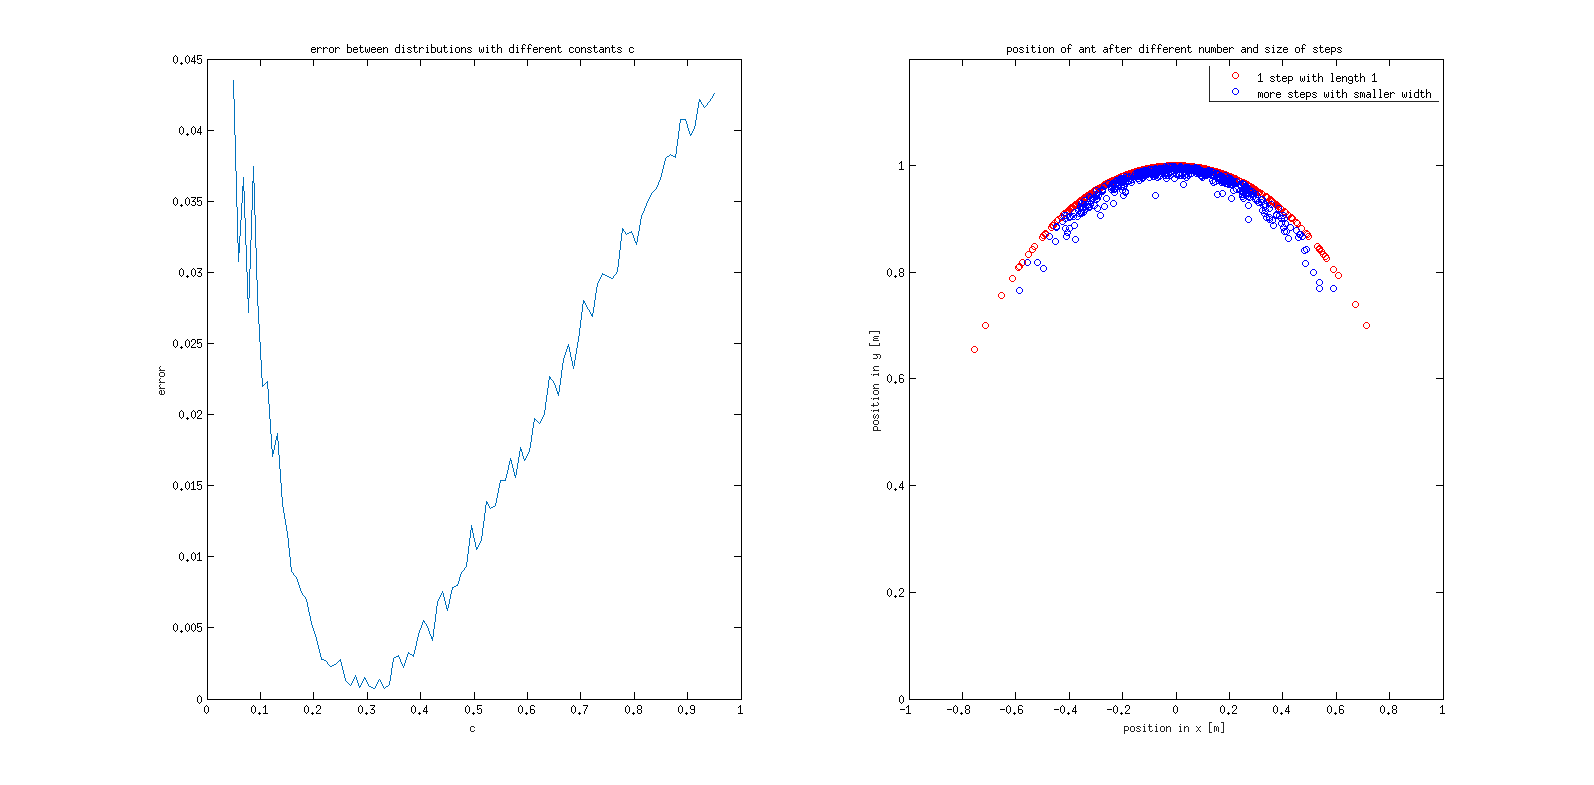
\includegraphics[scale=0.32]{./Pics/VarianceForStepWidth_plot.png} 
\caption{Variance for stepwidth \label{fig:Variance} }
\end{figure} 


\subsection{Verification of the Results}


To verify, if we implemented the path integrator correctly, we let the ants do the same experiment as described in Wehner1988 \cite{Wehner1988}.
The ant starts at the nest and walks 12 meters from the nest in a fixed direction. After that it turns an angle $\alpha$ and walks another 5 meters in this direction, where it finds food. At this point Wehner and Müller measured the angle the ants would take to find home and calculated the error in comparison to the exact position of the nest.
Our results produced look exactly the same, what indicates, that we implemented the path integrator in the way Wehner and Müller think it is correct.\\


\begin{figure}[h!]%
\begin{minipage}[t]{7.9 cm}
\centering
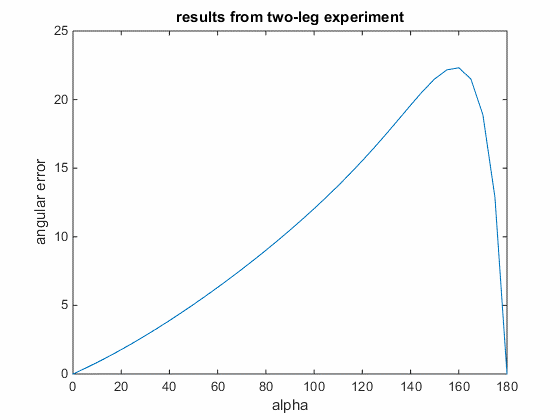
\includegraphics[scale=0.4]{./Pics/angularError.png} 
\caption{Angular Error produced \label{fig:AngErrorProd} }
\end{minipage}
%
\begin{minipage}[t]{7.9 cm}
\centering
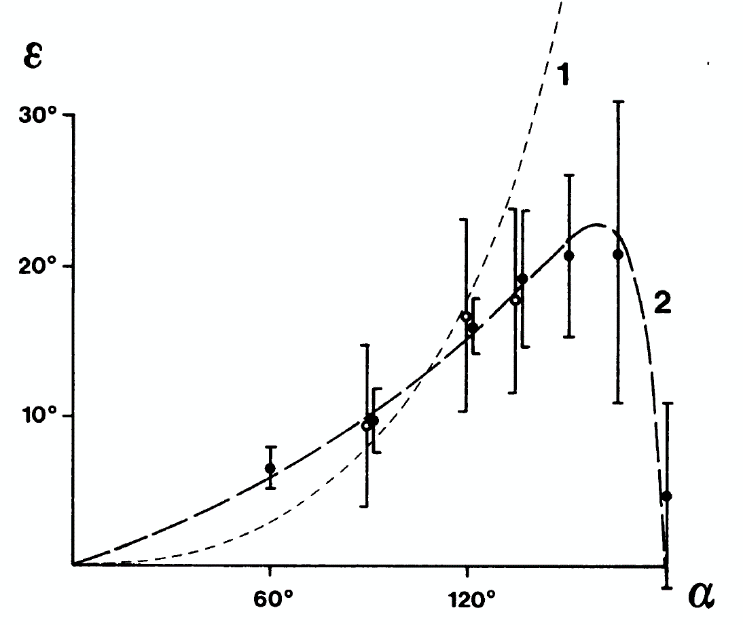
\includegraphics[scale=0.3]{./Pics/angularErrorOfWehner.png} 
\caption{Angular Error according to \cite{Wehner1988} \label{fig:AngErrorWehner} }
\end{minipage}
\end{figure}


In figure \ref{fig:AngErrorProd}, we see the angular error of our Matlab simulations. In figure \ref{fig:AngErrorWehner} we see the plot the paper Wehner1988\cite{Wehner1988}. Our implementation of the path integrator varies in the following points to the implementation of GordonTeam2008 \cite{GordonTeam2008}

\begin{itemize}
\item $\delta$ is meant as the angle between the angle of the global vector and the actual direction instead of the actual change in direction
\item the fitting constant k has to be rescaled if we use angles in radians instead of degrees.
\item they miscalculated the end of the second leg in the two-leg experiment.
\end{itemize}




\section{Summary and Outlook}
In the following section we would like to discuss our findings and provide an outlook on what could also be looked at in future projects.\\
\\ \\
\textit{Are we able to predict what happens if we alter the environment? (depends on the question beforehand) } \\ \\
We were able to run the simulation in different environments (different landmarks and variable food source locations). As a result we saw that the ants navigational behaviour strongly depends on the setup of the landmarks.
\\ \\ \\
\textit{Can the ants survive if we rid the environment completely of any landmarks?}
\\ \\
When the ant remains in radius of about ten meters around the nest it has no trouble to find back to the nest without the aid of visual landmarks. If the ants foraging radius reaches further, which in reality is often the case many ants will get lost along the way which makes landmarks essential at those distances. However, we do not know whether this also applies to real ants or if this effect is just an artifact of the employed model. This possibility cannot be dismissed since we used the model for a different purpose than it was originally designed for.
\\ \\ \\
In terms of the implemented model we were able to reproduce the error profile given by the experimental data in Wehner1988 \cite{Wehner1988} almost perfectly.

\newpage
\appendix
\section{Appendix}

\pagenumbering{roman}   % Macht Seitenzahl römisch





\subsection{run.m} \label{run}
\lstinputlisting[captionpos=b,caption=run.m,label="list:run.m"]{./Code/run.m}

\subsection{distanceBetweenTwoPoints.m}\label{distancebetweenTwoPoints}
\lstinputlisting[captionpos=b,caption=distanceBetweenTwoPoints.m,label="distanceBetweenTwoPoints.m"]{./Code/distanceBetweenTwoPoints.m}
\subsection{vector2angle.m}\label{vector2angle}
\lstinputlisting[captionpos=b,caption=vector2angle.m,label="list:vector2angle.m"]{./Code/vector2angle.m}
\subsection{updateGround.m}\label{updateGround}
\lstinputlisting[captionpos=b,caption=updateGround.m,label="list:updateGround.m"]{./Code/updateGround.m}
\subsection{Landmark.m}\label{Landmark}
\lstinputlisting[captionpos=b,caption=Landmark.m,label="list:Landmark.m"]{./Code/Landmark.m}
\subsection{Ground.m}\label{Ground}
\lstinputlisting[captionpos=b,caption=Ground.m,label="list:Ground.m"]{./Code/Ground.m}
\subsection{Ant.m}\label{Ant}
\lstinputlisting[captionpos=b,caption=Ant.m,label="List:Ant.m"]{./Code/Ant.m}

\newpage
\section{Declaration of originality}
\includegraphics[scale=0.7]{./Pics/Decleration.png}% 

\newpage


\section{Correspondence} \label{Sec:Correspondence}
R. Wehner ,author of \cite{Wehner2003},\cite{Wehner1988}, \cite{Wehner1998} kindly answered us a few questions.\\


\includegraphics[scale=0.5]{./Pics/email2.png}% 


\includegraphics[scale=0.8]{./RWehner.png}%


\section{References}
%-------------------------------------Bibliographie-------------------------------------
\bibliography{./Literatur}  
 %Zuerst muss man TexFile2 mal in ein PDF kompilieren, dann einmal Bibfile (F11), dann nochmal in ein PDF
 %\bibliographystyle{apalike}
  %\bibliographystyle{plain}
\bibliographystyle{abbrv}
\nocite{Wehner2008}
\nocite{Wehner2003}
\nocite{Wehner1988}
\nocite{GordonTeam2008}
\nocite{Mathworks2015}
%\nocite{Gebert2001}
\thispagestyle{plain}






\end{document}  



 
